\begin{frame}
    \frametitle{Cơ sở vector trong mặt phẳng}
    Với \(\mathbf{e}_1 ,\mathbf{e}_2\) không nằm trên cùng một đường thẳng,
    \[\mathbf{v}=a\mathbf{e}_1 +b\mathbf{e}_2 ; \qquad \mathbf{w}=c\mathbf{e}_1 +d\mathbf{e}_2 .\]
    Tổng của hai vector này \[\mathbf{v}+\mathbf{w}=(a+c)\mathbf{e}_1 +(b+d)\mathbf{e}_2 .\]
\end{frame}
\begin{frame}
    \frametitle{Toạ độ trên mặt phẳng-Mảng hai chiều}
    Những vector trên có thể được viết thành
    \begin{align*}
    \mathbf{v} &= (a,b),\\
    \mathbf{w} &= (c,d),\\
    \mathbf{v}+\mathbf{w} &= (a+c,b+d).
    \end{align*}
    \begin{itemize}
        \item Toạ độ của \(\mathbf{v}\) là \(v_1 =a\) và \(v_2 =b\).
        \item Toạ độ của \(\mathbf{w}\) là \(w_1 =c\) và \(w_2 =d\).
    \end{itemize}
\end{frame}
\begin{frame}
\frametitle{Cơ sở vector trong không gian}
\begin{columns}
\begin{column}{0.5\textwidth}
Với \(\mathbf{e}_1 ,\mathbf{e}_2 ,\mathbf{e}_3\) không cùng nằm trên một mặt phẳng, 
\begin{equation}
    \mathbf{u}=a\mathbf{e}_1+b\mathbf{e}_2+c\mathbf{e}_3
\end{equation}
\[\mathbf{u}=(u_1 ,u_2 ,u_3)=(a,b,c).\]
\end{column}
\begin{column}{0.5\textwidth}
\begin{figure}
\centering
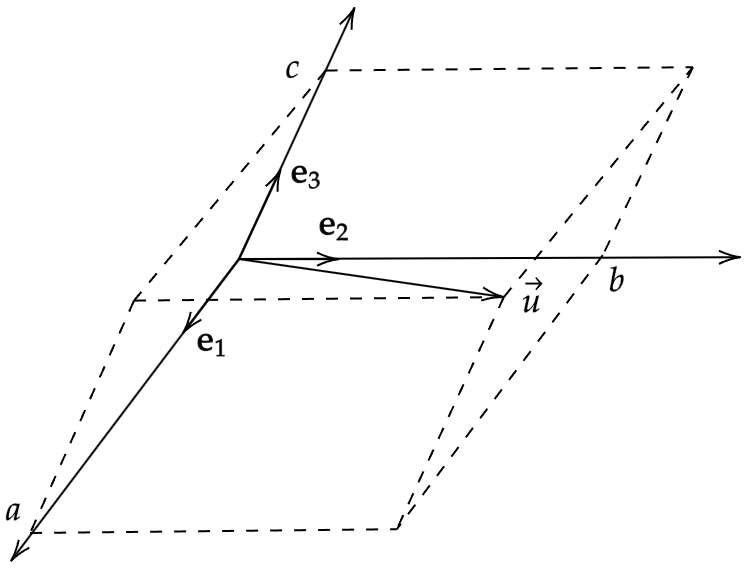
\includegraphics[width=0.9\textwidth]{Slides/Figure/cosovector.png}
\caption{Cơ sở \((\mathbf{e}_1, \mathbf{e}_2, \mathbf{e}_3)\)}
\end{figure}
\end{column}
\end{columns}
\end{frame}
\begin{frame}
\frametitle{Vector đơn vị}
\begin{tcolorbox}[colback=blue!10, colframe=blue!50!black, title=Định nghĩa]
    Một vector đơn vị là một vector có độ dài bằng 1:
\begin{equation}
    \mathbf{u} = \frac{\mathbf{a}}{|\mathbf{a}|} 
\end{equation}
Vector này  cùng hướng với \(\mathbf{a}\).
\end{tcolorbox}
\end{frame}

\begin{frame}
\frametitle{Hệ tọa độ Descartes}
\(\{\mathbf{e}_1 ,\mathbf{e}_2 ,\mathbf{e}_3\}\) là một tập hợp các vector trực chuẩn (trực giao và chuẩn hoá):
\[
        \mathbf{r}=\mathbf{OM} = x\mathbf{e}_1 + y\mathbf{e}_2 + z\mathbf{e}_3 =(x,y,z).
    \]
\begin{figure}
\centering
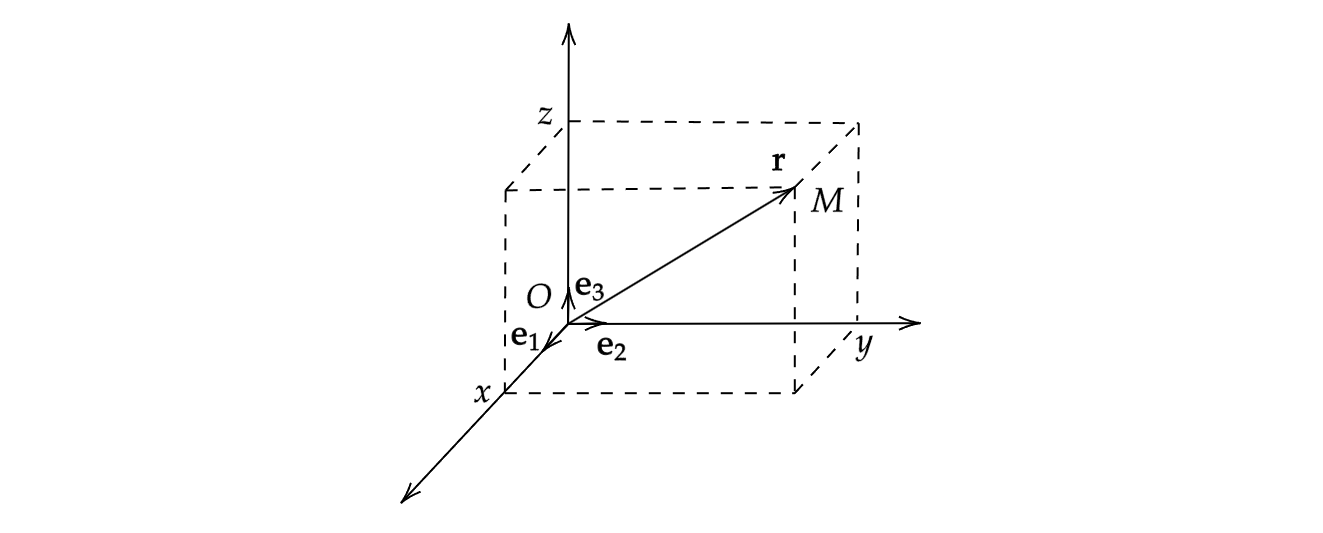
\includegraphics[width=12cm, height=4.5cm]{Slides/Figure/toadodescartes.png}
\caption{Hệ tọa độ Descartes \(Oxyz\)}
\end{figure}
\end{frame}

\begin{frame}
    \frametitle{Tính chất của hệ cơ sở trực chuẩn}
    Tích vô hướng của các vector cơ sở:
    \begin{equation*}
    \mathbf{e}_i \cdot \mathbf{e}_j =\delta_{ij}.
\end{equation*}Ký hiệu Kronecker: \begin{equation*}
\begin{array}{l}
     \delta_{ij}=\Bigg\{
    \begin{array}{ll}
      1  & \text{, nếu } i=j. \\
      0  & \text{, nếu } i\neq j.
    \end{array}
\end{array}
\end{equation*}
Do đó,
\begin{equation}
    \mathbf{a}\cdot\mathbf{b}= \sum_{i=1}^{3}\sum_{j=1}^{3}a_i b_j \delta_{ij}= \sum_{i=1}^{3} a_i b_i = a_1 b_1 + a_2 b_2 + a_3 b_3.
\end{equation}
\end{frame}
\begin{frame}
    \frametitle{Tính chất của hệ cơ sở trực chuẩn}
    Tích có hướng của các vector cơ sở:
    \begin{equation*}
        \mathbf{e}_i \times\mathbf{e}_j =\mathbf{e}_k \varepsilon_{ijk}.
    \end{equation*}
    Ký hiệu Levi-Civita:
    \begin{equation*}
\begin{array}{l}
        \varepsilon_{ijk}=\Bigg\{
        \begin{array}{ll}
        1  & \text{, nếu } (i,j,k)=(1,2,3) \text{ hoặc } (2,3,1) \text{ hoặc } (3,1,2).\\
        -1 & \text{, nếu } (i,j,k)=(1,3,2) \text{ hoặc } (2,1,3) \text{ hoặc } (3,2,1).\\
        0  & \text{, nếu } i=j \text{ hoặc } j=k \text{ hoặc } k=i.
        \end{array}
\end{array}
\end{equation*}
Do đó, 
\begin{equation}
    \mathbf{a} \times \mathbf{b} = \sum_{i=1}^{3}\sum_{j=1}^{3}\sum_{k=1}^{3}\varepsilon_{ijk} a_i b_j  \mathbf{e}_k.
\end{equation}
\end{frame}